In image processing the \textbf{Hough Transform} is useful for \textit{global} filtering, especially to find sets of pixels that lie along curves of a specified shape, i.e. finding lines, circles, ellipses, spheres, hypercubes, etc. It provides an elegant solution using a \textit{discretized parameter space}, while the na\"ive, brute-force approach quickly becomes daunting. In the case of finding lines in an image of $n$ points, the na\"ive approach involves iteration over all $\sim\!\! n^2$ possible lines and performing $\sim\!\! n^3$ comparisons for every point to each line. The $O(n^3)$  complexity exponentially worsens for shapes with higher dimensional parameter spaces. This approach is computationally prohibitive for non-trivial applications.

Instead, the Hough Transform accumulates non-background points in a discretized parameter space. The dimensionality of the parameter space is equal to the number of the parameters that describe the desired shape. In the case of a line, there are two parameters. However, the parameters must be defined with care. The na\"ive parameter choices for a line might be \textit{slope} and \textit{intercept}, but if the objective might include finding vertical (or nearly vertical) lines, a method to accurately discretize/store infinity (or very large values) would be required. A better approach is to parameterize lines by their \textit{normal} representation:
\begin{equation}
x \cos (\theta) + y \sin(\theta) = \rho \; . \label{eq:hough:line}
\end{equation}
In this parameterization, all parameters are nicely bounded: $-\sfrac{\pi}{2} \leq \theta \leq \sfrac{\pi}{2}$ and $-D\leq \rho \leq D$ for an image with D length between the two most distant corners.

The Hough Transform is a general algorithm, though in some cases it is analogous to formal mathematical transforms (eg. the Hough transform of lines with 'normal' parameterization is analogous to the Radon Transform). A typical pre-processing step for the image in question is edge detection to form a binary image, though this is not strictly necessary. The algorithm proceeds as follows:
\begin{enumerate}
	\item \label{item:houghalg:allocate} Allocate an accumulator image, selecting the appropriate number and width of bins for each parameter. 
	\item \label{item:houghalg:selectpixel} Select a foreground pixel.
	\item \label{item:houghalg:selectparam} Select center-of-bin values for (the same) $n-1$ of the $n$ parameters.
	\item \label{item:houghalg:solve} Solve for the final parameter value to satisfy the reference equation at the selected pixel.
	\item \label{item:houghalg:increment} Increment the accumulator image at the chosen- and solved- parameter location.
	\item \label{item:houghalg:iterparam} Repeat steps \ref{item:houghalg:selectparam} - \ref{item:houghalg:increment} for all possible chosen parameter values.
	\item \label{item:houghalg:iterpixel} Repeat steps \ref{item:houghalg:selectpixel} - \ref{item:houghalg:iterparam} for all foreground pixels in the image.
	\item \label{item:houghalg:findfeatures} Find parameters for prominent features by the location of accumulator maximum, or thresholding.
\end{enumerate}
In the case of non-binary images, the accumulator simply need not be discrete, such that foreground (or all) pixels just have a partial-voting effect. This algorithm simply extends to higher dimensional images, and higher dimensional parameter spaces. The complexity depends linearly upon the number of foreground pixels. 

As a concrete example, consider the binary image (with foreground as black)
\begin{center}
	\begin{tikzpicture}
\begin{axis}[title=Image, axis equal image, y dir=reverse, enlargelimits=false, tick style={draw=none}]
\addplot[patch,patch type=rectangle, color=black, faceted color=none]
coordinates {
	(0,0) (1,0) (1,1) (0,1) 
	(101, 101) (101,100) (100, 100) (100, 101)
	(101,0) (100,0) (100,1) (101,1)
	(0,101) (1,101) (1,100) (0,100) 
	(51,51) (51,50)(50,50)(50,51)
};
\end{axis}
	\end{tikzpicture}
\end{center}

By performing a Hough Transform with (\ref{eq:hough:line}) defining the parameters, and with the range of $\theta = \pm 90 ^{\circ}$ and $\rho = \pm \sqrt{2}C$, the resulting accumulator image is
\begin{center}
	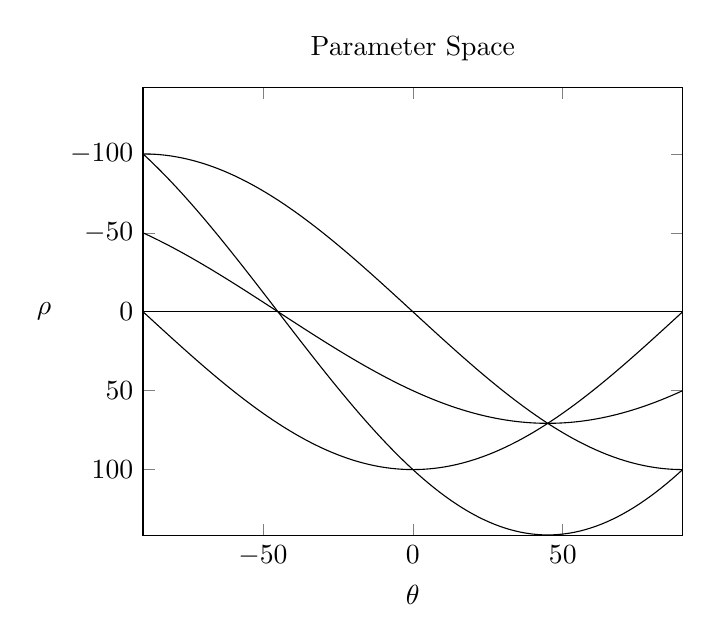
\begin{tikzpicture}
	\begin{axis}[title=Parameter Space, y dir=reverse, enlargelimits=false, ylabel=$\rho$,ylabel style={rotate=-90}, xlabel=$\theta$,xmin=-90,xmax=90,ymin=-142,ymax=142]
	\addplot[domain=-90:90, samples=101] {0* sin(x)};
	\addplot[domain=-90:90, samples=101] {100 * sin(x)};
	\addplot[domain=-90:90, samples=101] {70.7 * sin(x+45)};
	\addplot[domain=-90:90, samples=101] {100 * sin(x+90)};
	\addplot[domain=-90:90, samples=101] {141.4 * sin(x+45)};
	\end{axis}
	\end{tikzpicture}
\end{center}
(Realistically these sinusoids are just the patterns of the discrete bins, not actual sinusoidal curves, but I'm lazy and made 5 curves instead of $101^2$ boxes.) The locations where these curves intersect have accumulator values of 2 or 3 (however many curves intersect). From the intersection of the three curves at $(45, 70.7)$ and $(-45, 0)$, we conclude that there are three foreground points that lie on each lines diagonally across the image. Also notice how this special case of the Hough Transform is equivalent to the Radon Transform.